\documentclass[a4paper, twoside, 11pt]{report}
\usepackage[utf8]{inputenc}
\usepackage[francais]{babel}
\usepackage[T1]{fontenc}
\usepackage{lmodern}

\usepackage[footskip=2.7cm]{geometry}
\usepackage{lscape}
\usepackage{multicol}
%\usepackage{makeidx}
\usepackage{fancyhdr}
\usepackage{marvosym}
\usepackage{amsmath}
\usepackage{graphicx}
\usepackage{wrapfig}
\usepackage{amssymb}
\usepackage{listings}
\usepackage{subfigure}
\usepackage{wrapfig}
\usepackage{textcomp}
\usepackage{color}
\usepackage{supertabular}
\usepackage {setspace}
\RequirePackage[colorlinks=true,linkcolor=black]{hyperref}
%\usepackage{fullpage}

%\renewcommand{\rmdefault}{phv}

%Specifie le dossier des images
\graphicspath{{images/}}

%%Configuration de listings -----------------------------------
\lstset{%configuration de listings
float=hbp,%
basicstyle=\ttfamily\small, %
identifierstyle=\color{colIdentifier}, %
keywordstyle=\color{colKeys}, %
stringstyle=\color{colString}, %
commentstyle=\color{colComments}, %
columns=flexible, %
tabsize=2, %
frame=trBL, %
frameround=tttt, %
extendedchars=true, %
showspaces=false, %
showstringspaces=false, %
numbers=left, %
numberstyle=\tiny, %1
breaklines=true, %
breakautoindent=true, %
captionpos=b,%
xrightmargin=0cm, %
xleftmargin=-0cm, %
language=tex, %
frameround=fttt;%
}
%%Fin de la configuration de listings -----------------------------------

\newcommand{\couverture}[0]{
  \thispagestyle{
    \fancyhf{}
    \renewcommand{\footrulewidth}{0pt}
    \renewcommand{\headrulewidth}{0pt}
  }
  \begin{picture}(0,0)
    \put(0,-220){\includegraphics[width=15cm]{logoCle.png}} %pour mettre une image de fond qui sera recouverte.
    \put(-75,-755){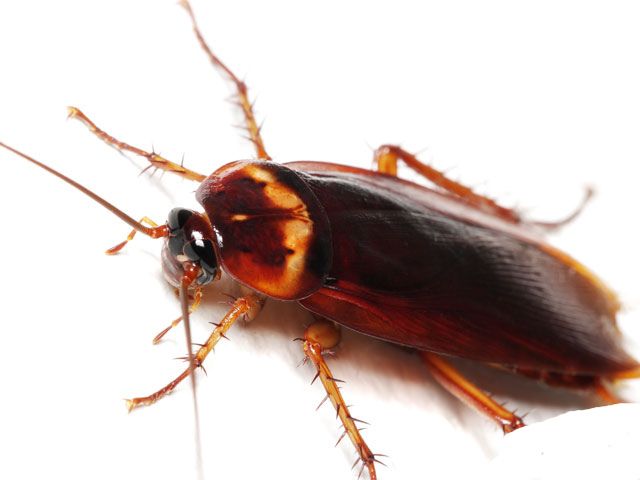
\includegraphics[width=211mm]{blatte.jpg}}
    \put(140,-620){\begin{minipage}{13cm} \Large Blatte War\end{minipage}}
    \put(-65,-600){\begin{minipage}{6.3cm} \Large \raggedleft Projet d'informatique répartie\end{minipage}}
    \put(370,-750){\begin{minipage}{5cm} \raggedleft \footnotesize version 1.00 \end{minipage}}
  \end{picture}
}

%\makeindex

%Design de la couverture
\def\thickhrulefill{\leavevmode \leaders \hrule height 1pt\hfill \kern \z@}
\def\maketitle{%
  \thispagestyle{empty}%
  \begin{picture}(0,0)
    \put(-35,-300){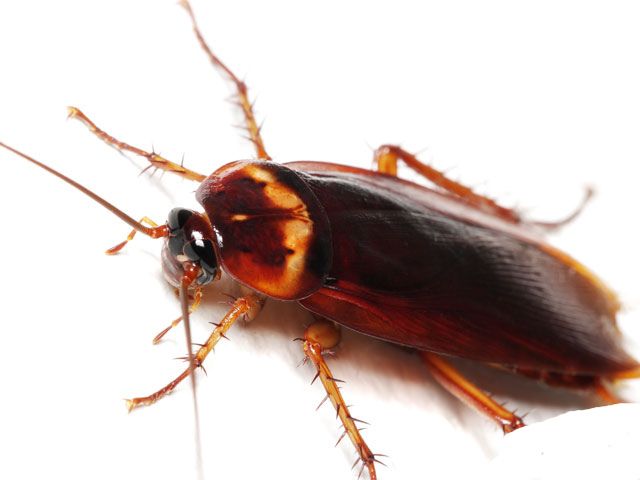
\includegraphics[width=17cm]{blatte.jpg}} %pour mettre une image de fond qui sera recouverte.
    \put(-100,-775){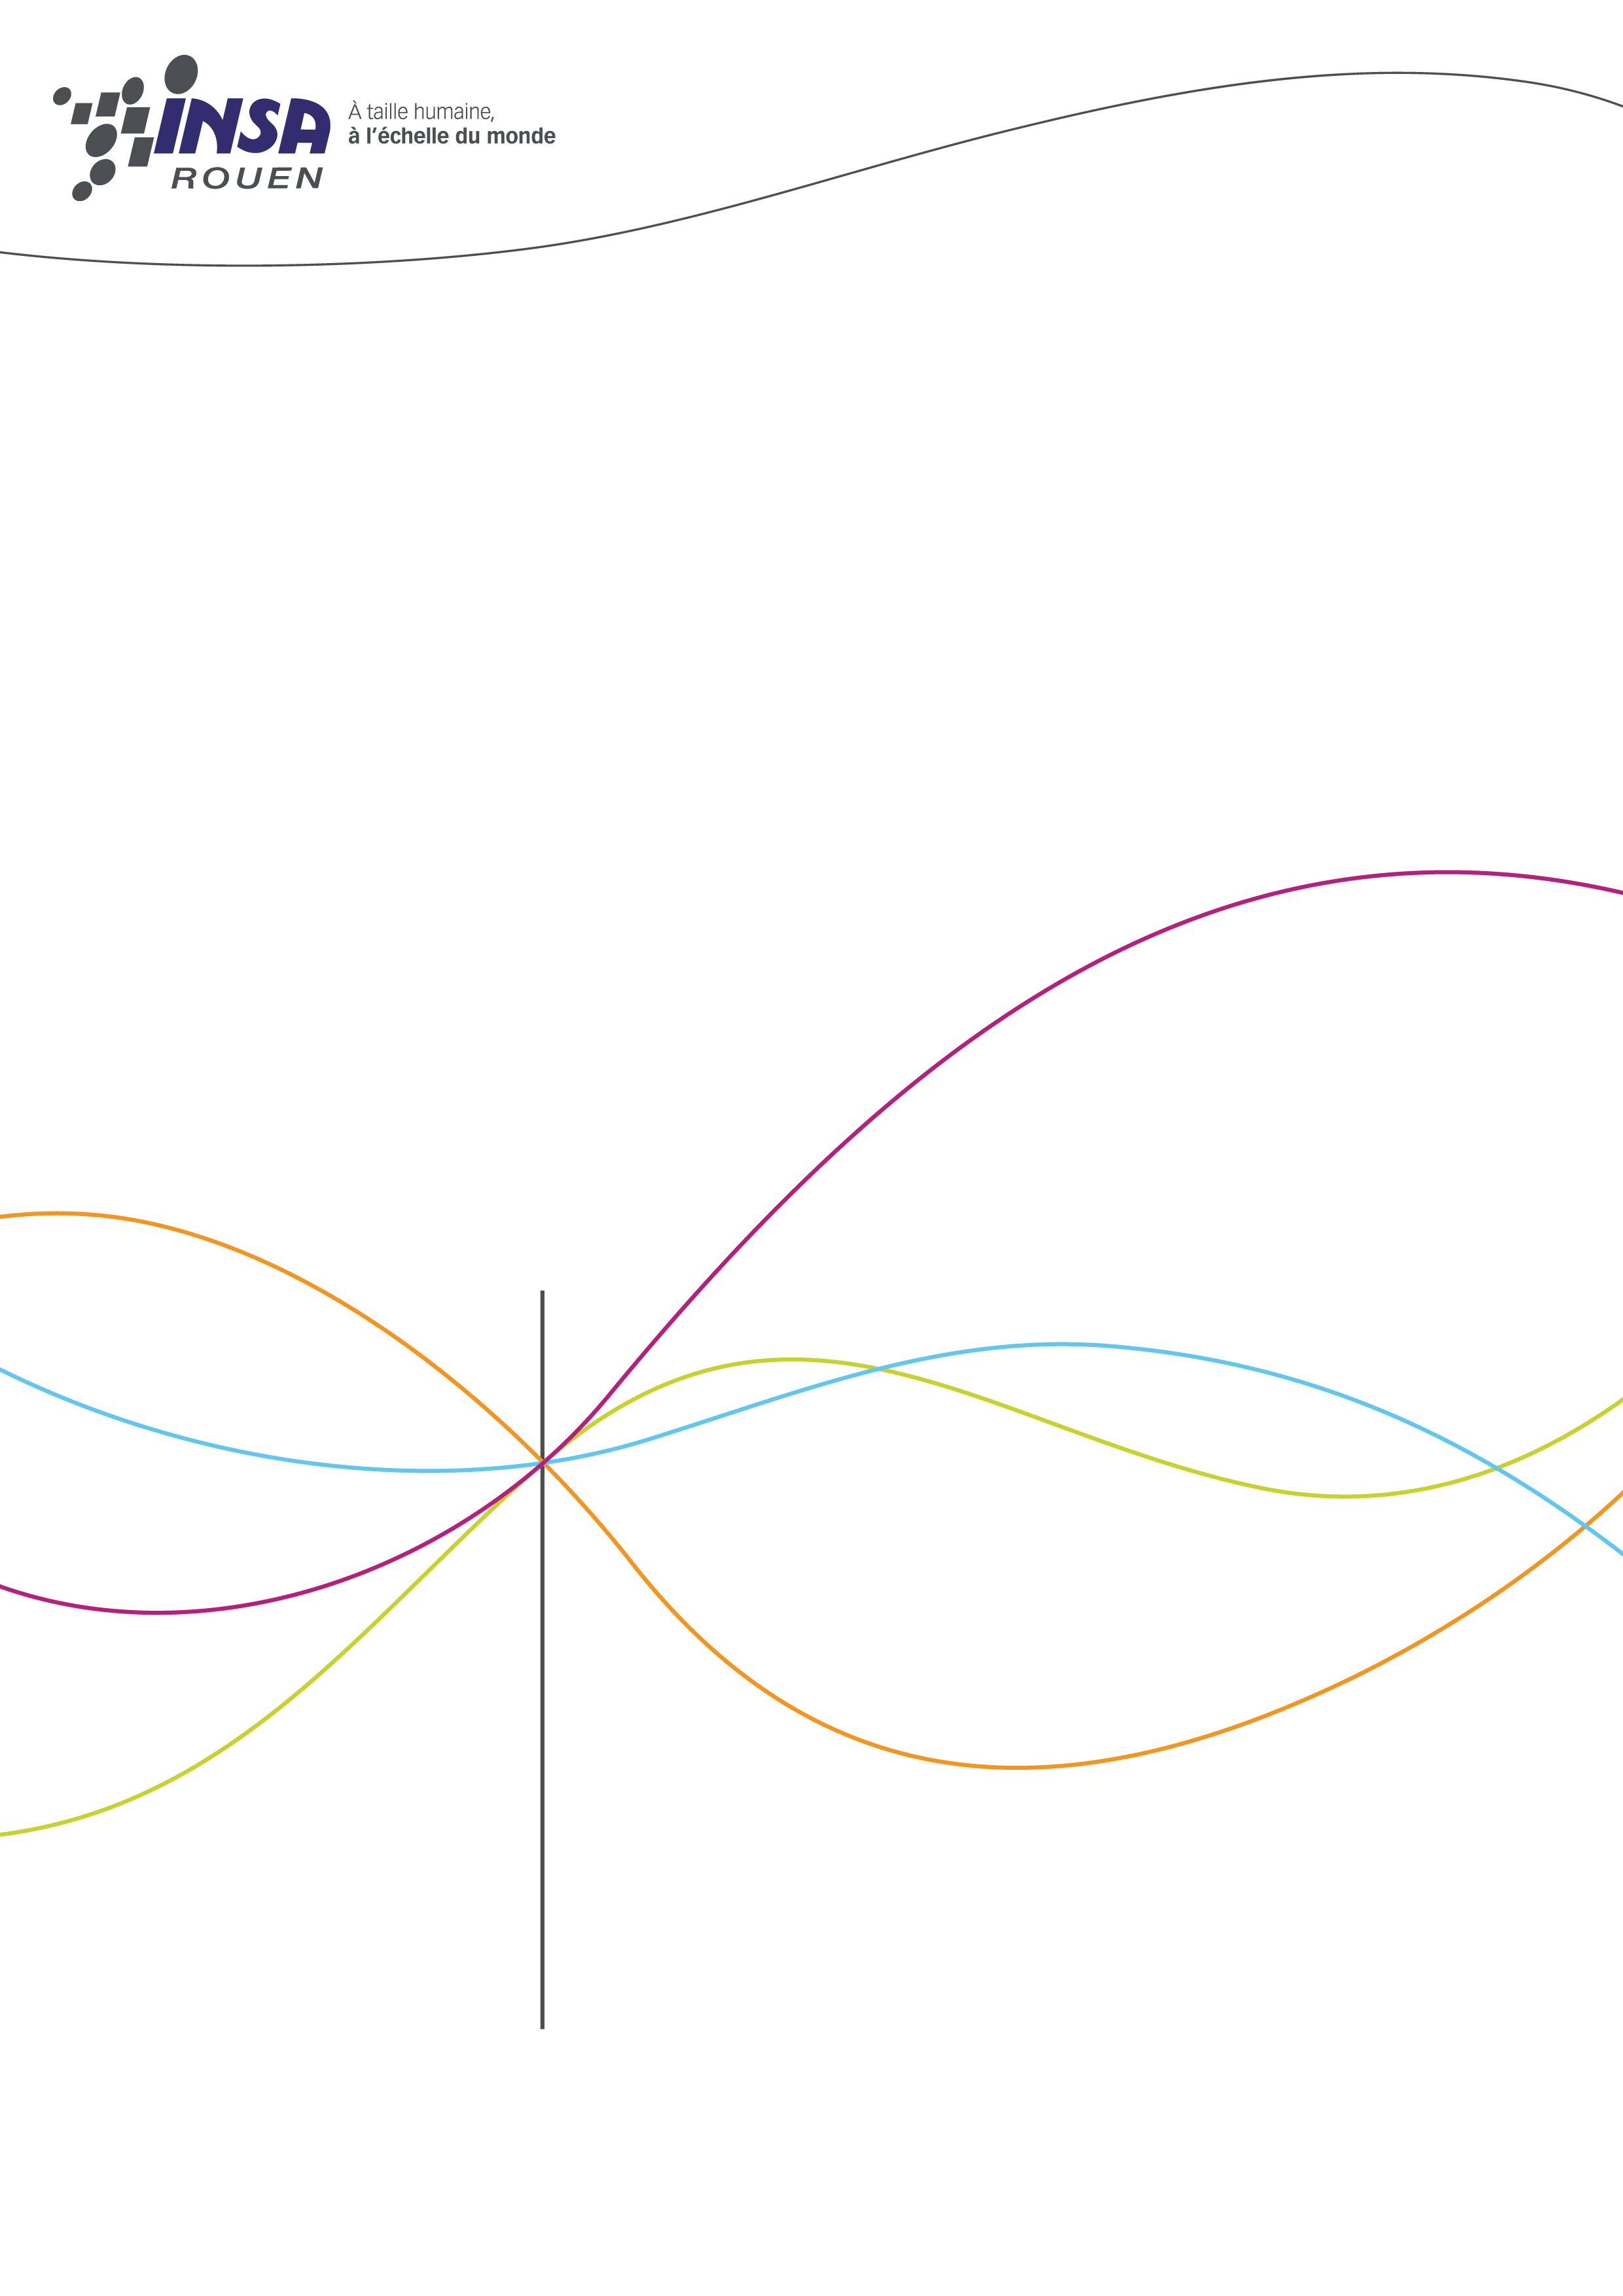
\includegraphics[width=211mm]{couverture.png}}
    \put(110,-620){\begin{minipage}{13cm} \large Projet d'informatique répartie \\ \huge Blatte War \end{minipage}}
    \put(-90,-620){\begin{minipage}{6.3cm} \Large \raggedleft Bienaimé Pierre\\Bonnet Bastien\\Chataigner Mathieu\\Fresquet Mathieu\\Meuleman Pâris \\Parès Yves\\Reiter Thibaut\\ \end{minipage}}
    \put(350,-750){\begin{minipage}{5cm} \footnotesize À l'attention de A.Pauchet \end{minipage}}
  \end{picture}
  \clearpage
}

%En-tete et pied de page
\setlength{\headheight}{15pt}
\pagestyle{fancy}
\renewcommand{\headrulewidth}{0.3pt}
\renewcommand{\footrulewidth}{0.3pt}
\lhead{\leftmark{}}
\rhead{Blatte War}
\definecolor{colKeys}{rgb}{0,0,1}
\definecolor{colIdentifier}{rgb}{0,0,0}
\definecolor{colComments}{rgb}{0,0.5,1}
\definecolor{colString}{rgb}{0.6,0.6,0.1}
\lfoot{Projet d'informatique répartie}
\cfoot{\thepage}
\rfoot{
\includegraphics[width=2cm,height=0.7cm]{logoASI.pdf}}

%\sloppy
%\interfootnotelinepenalty=150 %note de bas de page
%\widowpenalty=150
%\clubpenalty=150 
%\setlength{\parindent}{15mm}


%%%% debut macro pour enlever le nom chapitre %%%%
% \makeatletter
% \def\@makechapterhead#1{%
%   \vspace*{50\p@}%
%   {\parindent \z@ \raggedright \normalfont
%     \interlinepenalty\@M
%     \ifnum \c@secnumdepth >\m@ne
%         \Huge\bfseries \thechapter\quad
%     \fi
%     \Huge \bfseries #1\par\nobreak
%     \vskip 40\p@
%   }}
% \def\@makeschapterhead#1{%
%   \vspace*{50\p@}%
%   {\parindent \z@ \raggedright
%     \normalfont
%     \interlinepenalty\@M
%     \Huge \bfseries  #1\par\nobreak
%     \vskip 40\p@
%   }}
% \makeatother
%%%% fin macro %%%%



\parskip=5pt

\begin{document}

\maketitle
\clearpage

\tableofcontents
\clearpage

\begin{onehalfspace}

  \chapter*{Introduction}
\addcontentsline{toc}{chapter}{Introduction}
\thispagestyle{fancy}
\lhead{Introduction}

Le présent document constitue le rapport de projet d'informatique répartie. Ce projet a pour objectif pédagogique de réutiliser et d'appliquer les connaissances des technologies étudiées au cours du semestre dans le cours d'informatique répartie.

~

Le principe de l'application répartie conçue dans ce projet consiste en un jeu d'arène où divers clients peuvent tester leur IA les uns contre les autres.

Chaque client dispose d'un personnage, appelé \og{}blatte\fg{}, interagissant avec son environnement et les autres blattes. L'arène est composé de cases qui peuvent posséder des propriétés diverses utilisables par les blattes.


  \chapter{Cahier Des Charges}
%\addcontentsline{toc}{chapter}{Cahier Des Charges}
\thispagestyle{fancy}
\lhead{Cahier Des Charges}

\section{Description de l'application}
    Il s'agit d'une application répartie de type client/serveur. Les joueurs connectent leur clients au serveur, ce qui leur permet de mesurer leur Intelligence Artificielle (IA) à celles des autres joueurs.
    
    Chaque joueur incarne une blatte dans le jeu. Les blattes évoluent dans une arène de type labyrinthe rectangulaire, constituée de cases pouvant être des obstacles (murs) ou des emplacements sur lesquels peuvent se trouver les blattes. Des objets disposant de propriétés particulières utilisables par les blattes peuvent se trouvent sur les cases libres (exemple : mine antipersonnel).

\section{Liste des fonctionnalités du produit final}
     \subsection{L'architecture de l'application}
         L'application doit fournir les fonctionnalités suivantes :
         \begin{itemize}
             \item Une interface doit permettre aux utilisateurs d'implémenter leur blatte ;
             \item Le serveur doit permette à des clients implémentant l'interface correspondant à une blatte de se connecter ;
             \item Le serveur doit gérer tout ce qui concerne l'architecure de l'arène ;
             \item Le serveur gère les interactions entre les blattes, le début et fin de partie, ainsi que les différentes phases de celle-ci.
         \end{itemize}
         
\newpage
    \subsection{Le jeu}
        Le jeu doit respecter les points suivants : 
        
        \paragraph{L'arène :}
        \begin{itemize}
            \item L'\texttt{arène} est supportée par le serveur;	
            \item L'arène est constituée de cases dont certaines sont murées (impossibles à traverser);	
            \item Chaque client présente une unique \texttt{blatte} contrôlée par une IA sur le terrain;
            \item Une case non murée de l'arène représente la case de victoire (non nécessairement bord de l'arène);
            \item Certaines cases non murées représentent des points de "Respawn" ou "Départ" (Lorsqu'une blatte meurt, elle peut réapparaître dessus);
            \item Une case peut posséder une propriété affectant la blatte se trouvant sur elle ;
            \item Les conditions de victoire pour un joueur sont la survie de sa blatte ou l'arrivée d'une blatte sur la case de victoire;
            \item Jeu au tour par tour, chaque client décide sa prochaine action et l'envoie au serveur avant que ce dernier n'effectue toutes les actions (ordonnancement des actions à définir).
        \end{itemize}
        
        \paragraph{Les blattes :}
        \begin{itemize}
            \item Chaque blatte a un nombre défini de vies et voit uniquement une case dans les 4 directions (avant, arrière, côté gauche, droit);
            \item Les actions possibles d'une blatte sont :
                \begin{itemize}
                    \item Avancer d'une case;
                    \item Attaquer au corps à corps;
                    \item Passer son tour;
                \end{itemize}
            \item La rencontre de deux blattes sur une même case entraîne obligatoirement la mort d'une des deux;
            \item Le serveur envoie au client à chaque tour une portion de map vue par la blatte;
            \item Chaque client envoie au serveur le coup joué.
        \end{itemize}



  \chapter{Conception Préliminaire}
%\addcontentsline{toc}{chapter}{Conception Préliminaire}
\thispagestyle{fancy}
\lhead{Conception Préliminaire}

\section{Diagramme du cas d'utilisation}

Ci-dessous se trouve le diagramme présentant le cas d'utilisation présentant le déroulement d'une partie:
    
\begin{figure}[h!]
\begin{center}
\includegraphics[width=.8\linewidth]{../conception/CasDUtilisation.pdf}
\caption{Cas d'Utilisation du déroulement d'une partie}
\end{center}
\end{figure}


\newpage
\section{Diagramme de séquence système}
Ci-dessous se trouve le diagramme de séquence système illustrant le cas d'utilisation présenté précédemment:
\begin{figure}[h!]
\begin{center}
\includegraphics[width=.8\linewidth]{../conception/DSS.pdf}
\caption{DSS du déroulement d'une partie}
\end{center}
\end{figure}

\newpage
\section{Maquettes}
Notre interface web permet de visualiser une partie en cours. Elle n'est constituée que d'une unique page. Voici une maquette de cette page:

\begin{figure}[h!]
\begin{center}
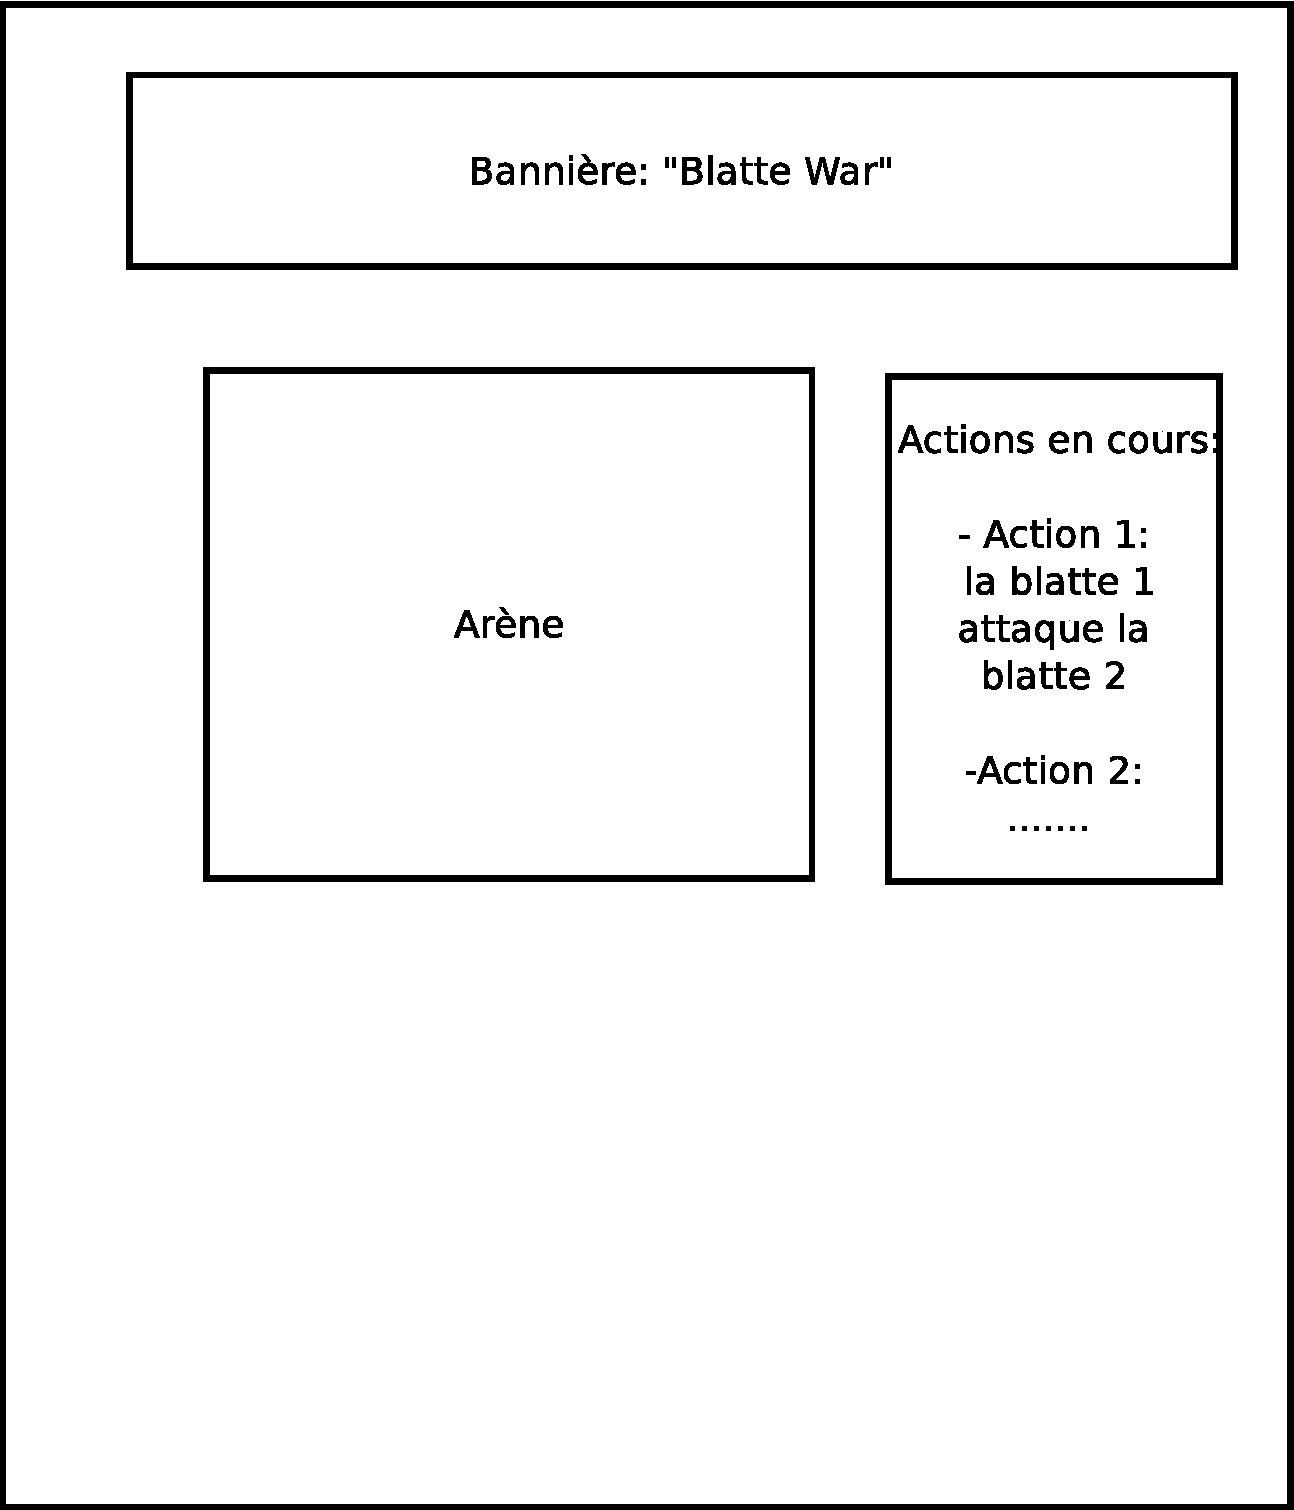
\includegraphics[width=.8\linewidth]{images/mockup.pdf}
\caption{Maquette de la page web (affichage de l'arène d'une partie en cours)}
\end{center}
\end{figure}


    
\newpage
\section{Diagramme de classe}
    L'implémentation du jeu devra respecter le diagramme de classe suivant :

    \begin{figure}[ht]
    \begin{center}
    \includegraphics[scale=0.32]{../conception/UML_Blatte.pdf}
    \end{center}
    \caption{Diagramme de classes, partie 1}
    \end{figure}

    \begin{figure}[ht]
    \begin{center}
    \includegraphics[scale=0.32]{../conception/UML_Blatte_p2.pdf}
    \end{center}
    \caption{Diagramme de classes, partie 2}
    \end{figure}


  \chapter{Développement}
\thispagestyle{fancy}
\lhead{Développement}

    \section{Méthode de développement}
            
        Après avoir réfléchi en groupe complet à l'établissement du cahier des charges, pour lequel il a fallu faire le tri entre de nombreuses idées afin de pouvoir réaliser le prototype dans les temps, défini les spécifications, nous devions nous hâter afin de pouvoir espérer finir dans les temps.

        Au vu du temps imparti, au cours des parties conception, développement et tests unitaires, nous avons répartis les effectifs de l'équipe sur des fonctionnalités de jeux relativement indépendantes afin de paralléliser les tâches. Ainsi, certains pouvaient commencer la création de l'arène pendant que d'autres s'occupaient de la gestion répartie (echanges client-serveur) comprenant aussi l'interface web. L'intérêt de cette modularité résidait essentiellement sur le fait que chacun pouvait travailler à son rythme (plutôt la journée ou plutôt le soir). 

    \section{Objectifs atteints}
            
        Nous avons réalisé la globalité des fonctionnalités demandées dans le cahier des charges.  
            
    %\section{Objectifs non-atteints}
        % Il n'y en aura pas !
    
    
    
    \section{Aperçu de l'interface web}
    
    Voici une capture d'écran de notre interface web permettant de visualiser une partie en cours. Caque joueur peut ainsi suivre l'évolution de sa blatte, dont il a programmé l'intelligence artificielle. Il est à noter que les observateurs peuvent modifier les couleurs et l'apparence de l'arène.
    De plus, plusieurs arènes différentes ont été implantées, mais à l'heure actuelle, nous n'avons pas encore offert la possibilité de permuter de l'une à l'autre facilement.

~
    
    \begin{figure}[h!]
\begin{center}
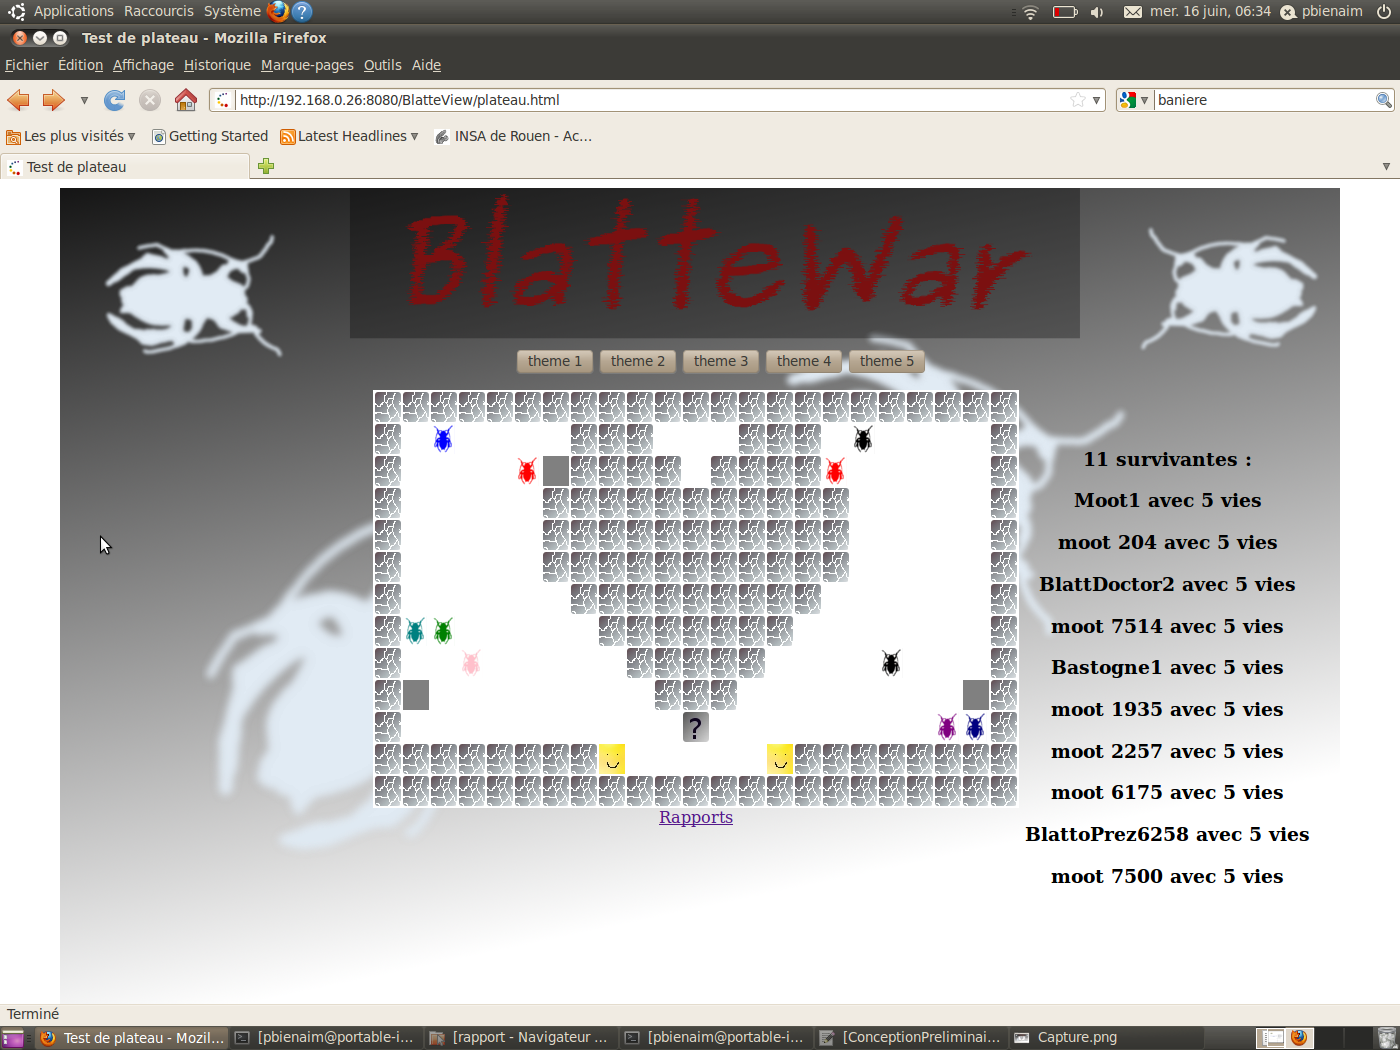
\includegraphics[width=.8\linewidth]{images/screenshot1.png}
\caption{Arène d'une partie en cours}
\end{center}
\end{figure}

    ~
    
    Enfin, il est possible de consulter les rapports complets de tous les matchs effectués, avec le détail de chaque action effectue par chaque blatte. Voici par exemple un extrait d'un rapport.
    
   \begin{figure}[h!]
\begin{center}
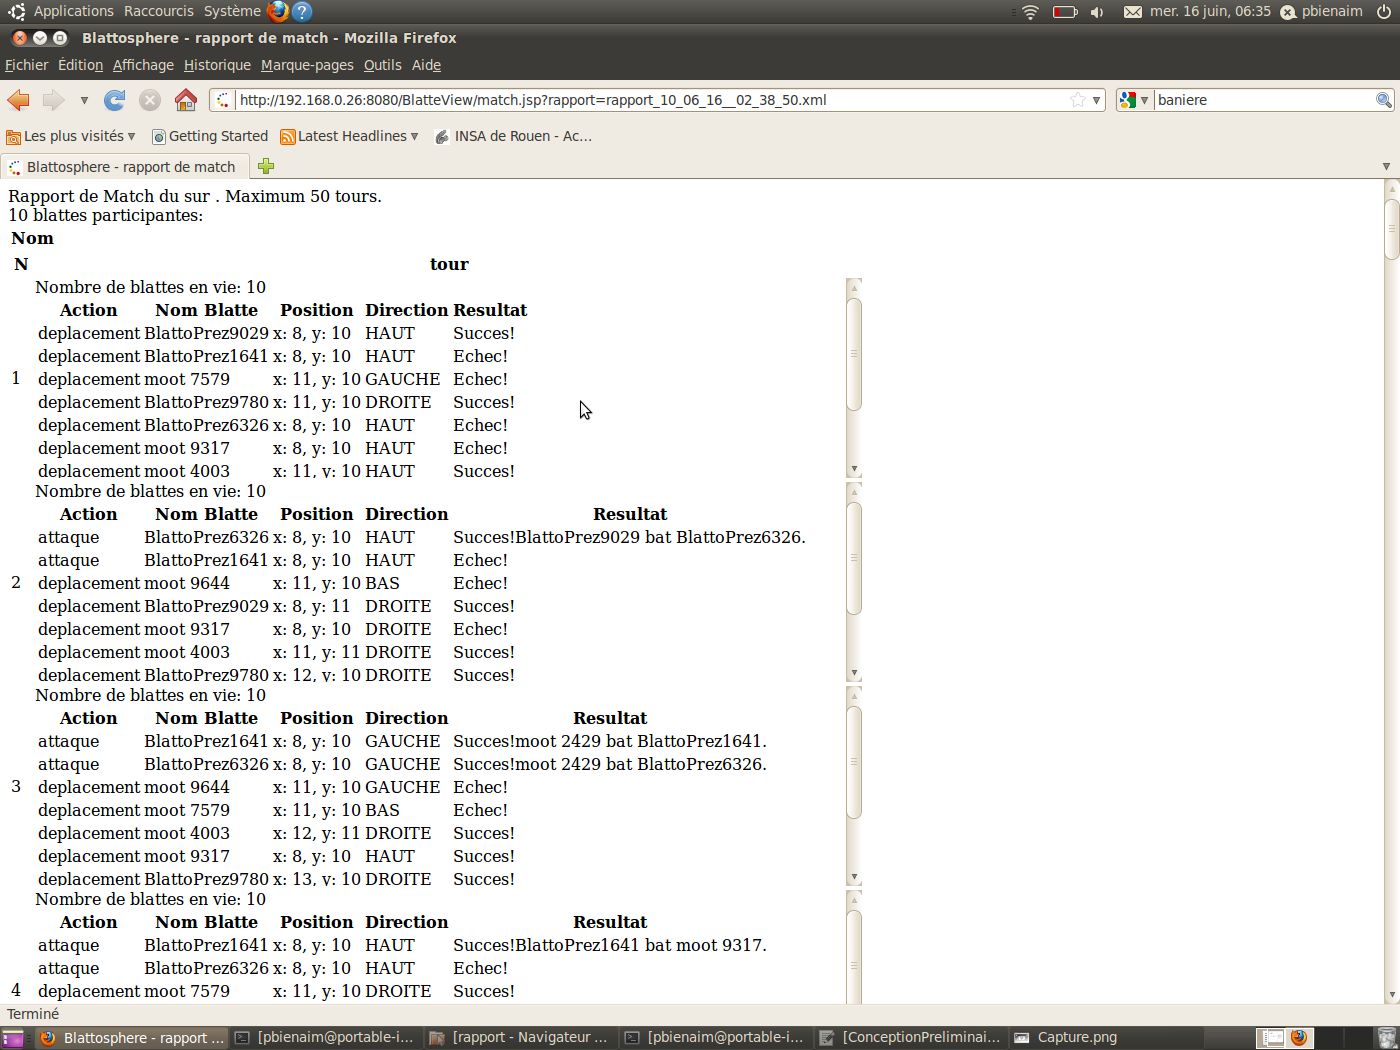
\includegraphics[width=.8\linewidth]{images/screenshot2.png}
\caption{Visualisation d'un rapport}
\end{center}
\end{figure}

 

  \chapter*{Conclusion}
\addcontentsline{toc}{chapter}{Conclusion}
\thispagestyle{fancy}
\lhead{Conclusion}

Ce projet nous a permis de consolider nos connaissances de base en technologie EJB en développant un applcation complexe (par comparaison avec ce que nous avons fait en TP).

Ils nous a également permis de réustiliser des connaissances acquises dans d'autres cours d'ASI, comme Algorithmique, Document et Programmation avancée.

Ce que nous retenons de ce projet est que notre choix d'intégration très progressive des composants nous a permis de gagner du temps par rapport à d'autres projets de même envergure que nous avons eu l'occasion de réaliser par le passé, comme le projet de Technologies Web du semestre précédent.

  
\end{onehalfspace}

\newpage
\thispagestyle{empty}
\begin{picture}(0,0)
  \put(-100,-755){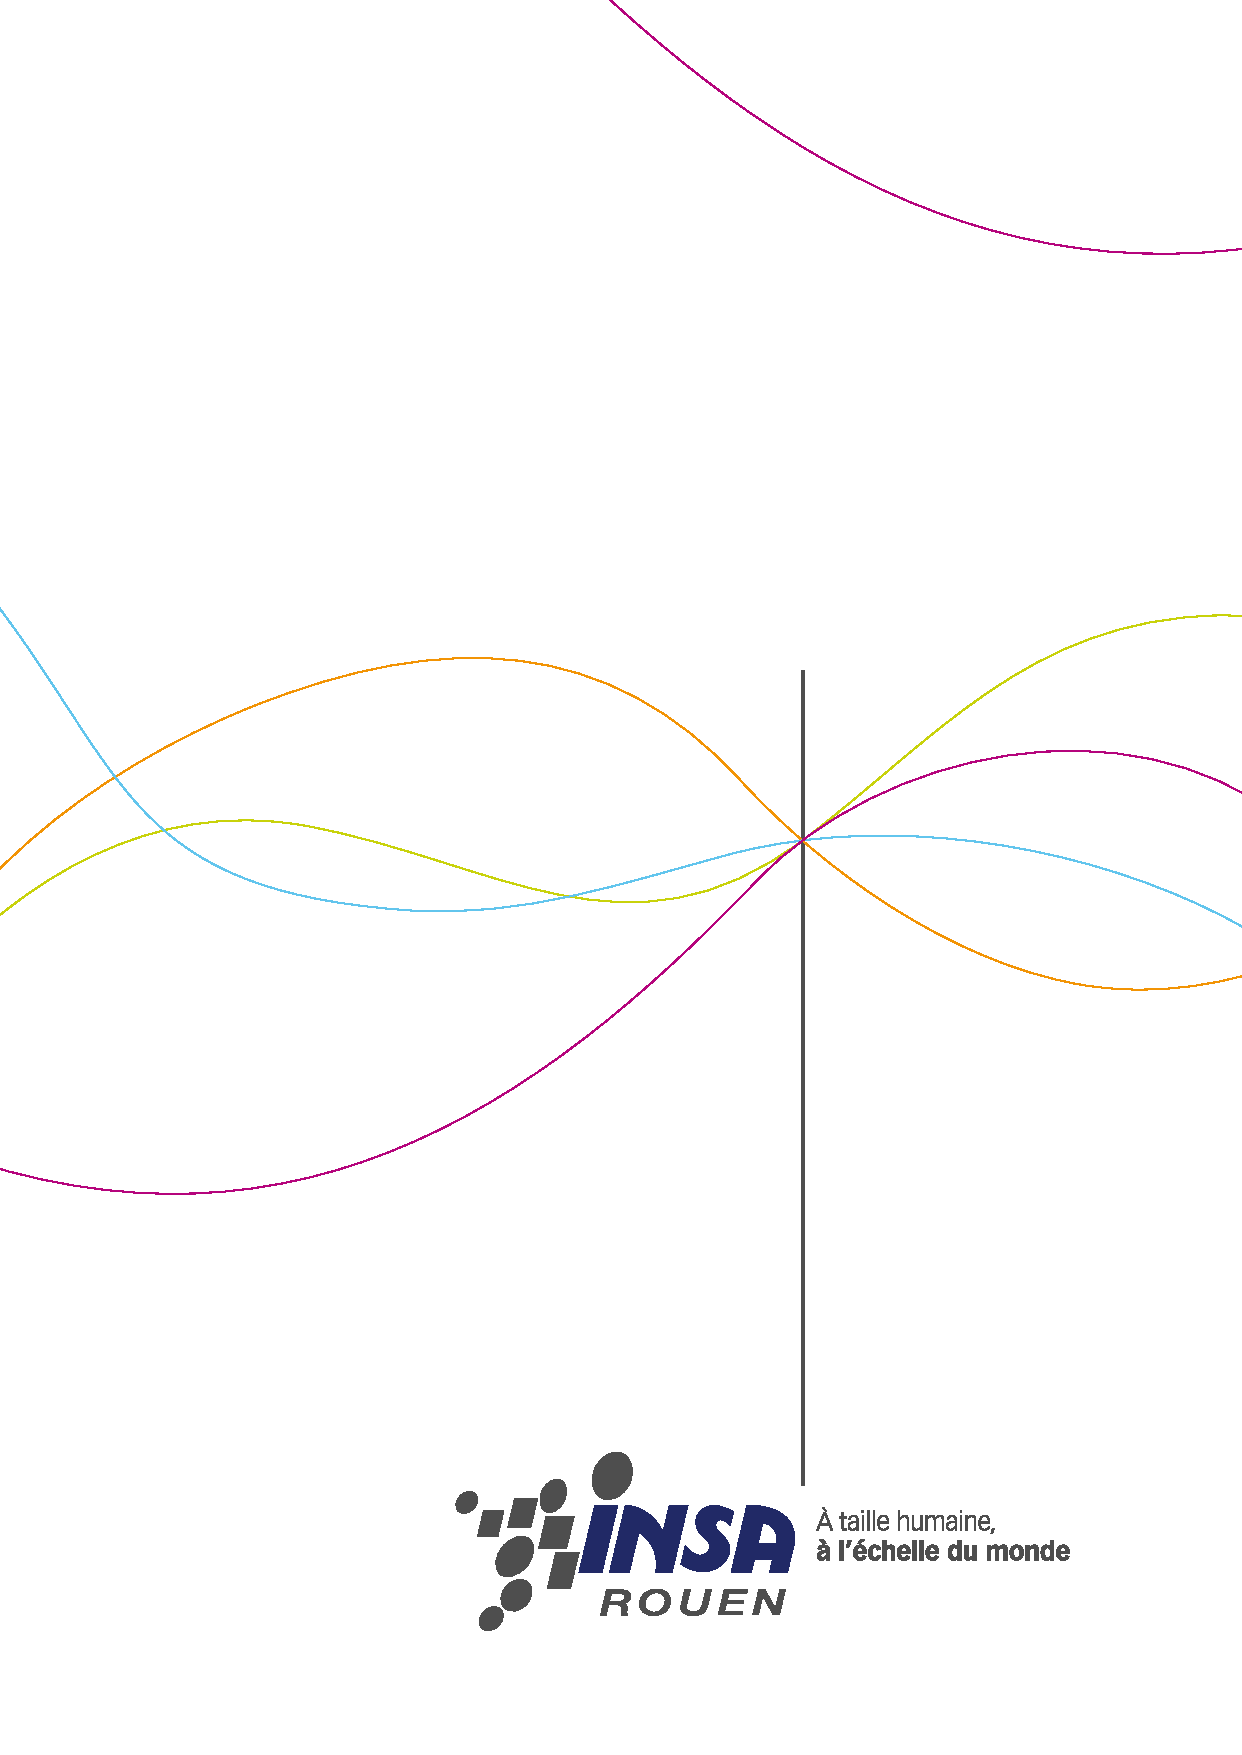
\includegraphics[width=211mm]{couvertureBis.pdf}}
  \put(60, -550){
    \begin{normalsize}
      \begin{minipage}{10cm}
        \begin{tabular}{r}
          INSA de Rouen\\
          Avenue de l'Université - BP 08\\
          76801 Saint-Etienne-du-Rouvray Cedex\\
          Tél : 02 32 95 97 79\\
          Fax : 02 32 95 97 08\\
          \textit{http://asi.insa-rouen.fr}\\
        \end{tabular}
      \end{minipage}
    \end{normalsize}}
  \put(300, -570){
\includegraphics[scale=0.4]{logoASI.pdf}}
\end{picture}

\end{document}
